\documentclass[tikz,border=6pt]{standalone}
\usepackage{amsmath}
\usetikzlibrary{arrows.meta,calc,patterns,positioning}
\begin{document}

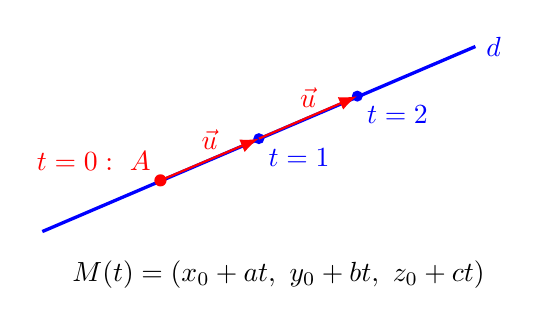
\begin{tikzpicture}[>=Latex,scale=1]
  \draw[blue,very thick] (-0.3,0.2) -- (5.2,2.55) node[right] {$d$};
  \coordinate (A) at (1.2,0.85);
  \coordinate (Mone) at (2.45,1.38);
  \coordinate (Mtwo) at (3.7,1.92);
  \fill[red] (A) circle (2.2pt) node[above left] {$t=0:\ A$};
  \fill[blue] (Mone) circle (2pt) node[below right] {$t=1$};
  \fill[blue] (Mtwo) circle (2pt) node[below right] {$t=2$};
  \draw[->,red,thick] (A) -- (Mone) node[midway,above] {$\vec u$};
  \draw[->,red,thick] (Mone) -- (Mtwo) node[midway,above] {$\vec u$};
  \node[align=left] at (2.7,-0.35) {$M(t)=(x_0+at,\ y_0+bt,\ z_0+ct)$};
\end{tikzpicture}

\end{document}
